\documentclass[11pt]{article}
\usepackage[margin=1in]{geometry}
\usepackage{graphicx}
\usepackage{booktabs}
\usepackage{hyperref}
\usepackage{longtable}
\usepackage{array}
\usepackage{xcolor}
\usepackage{listings}
\usepackage{fancyvrb}

\hypersetup{
  colorlinks=true,
  linkcolor=blue!50!black,
  urlcolor=blue!50!black
}

\lstset{
  basicstyle=\ttfamily\small,
  breaklines=true,
  frame=single,
  framerule=0.2pt
}

\title{newspaper-parsing: End-to-End Pipeline Walkthrough}
\author{Saul Richardson + Codex}
\date{February 13, 2026}

\begin{document}
\maketitle

\section{Goal}
This repository formalizes a single production pipeline for newspaper parsing:
\begin{itemize}
  \item Paddle layout detectors: \texttt{PP-DocLayoutV2}, \texttt{PP-DocLayoutV3}, \texttt{PP-DocLayout\_plus-L}
  \item Paddle VL parser: \texttt{doc\_parser v1.5}
  \item Dell layout parser
  \item MinerU2.5 layout parser
  \item Fusion with anti-noise gating
  \item Fused-region transcription with Paddle OCR
\end{itemize}

\section{Pipeline Stages}
\begin{enumerate}
  \item \texttt{paddle\_layout}
  \item \texttt{paddle\_vl15}
  \item \texttt{dell}
  \item \texttt{mineru}
  \item \texttt{fusion}
  \item \texttt{review}
  \item \texttt{transcription}
\end{enumerate}

\noindent
Transcription is ROI-first: Paddle OCR runs on a cleaned non-redundant subset of fused
\texttt{text/title} boxes, then OCR lines are remapped to page coordinates and serialized in fused reading order.

Run all stages:
\begin{lstlisting}
newsbag run --config configs/pipeline.torch.json \
  --stages paddle_layout,paddle_vl15,dell,mineru,fusion,review,transcription
\end{lstlisting}

\section{Torch Execution Pattern}
Recommended orchestration on Torch is a three-job chain:
\begin{enumerate}
  \item GPU inference (\texttt{l40s\_public} or split-L40S/H200): layout sources only
  \item CPU post-processing (\texttt{cs}): fusion and review bundles
  \item GPU transcription (\texttt{l40s\_public}): Paddle OCR over fused regions
\end{enumerate}

This structure avoids low-GPU-utilization cancellation by keeping CPU-only steps off GPU partitions.

\section{Case Study: 2-Page Mini Run (Corrected Dell)}
\textbf{Run ID:} \texttt{layout\_bagging\_20260213\_024626}\\
\textbf{Pages:}
\begin{itemize}
  \item \texttt{abilene-reporter-news-apr-29-1946-p-19}
  \item \texttt{bakersfield-californian-aug-31-1937-p-14}
\end{itemize}

\subsection{Visual Outputs}
\begin{figure}[h]
\centering
\includegraphics[width=0.92\textwidth]{images/mini_run/abilene_input.png}
\caption{Mini run input page (Abilene).}
\end{figure}

\begin{figure}[h]
\centering
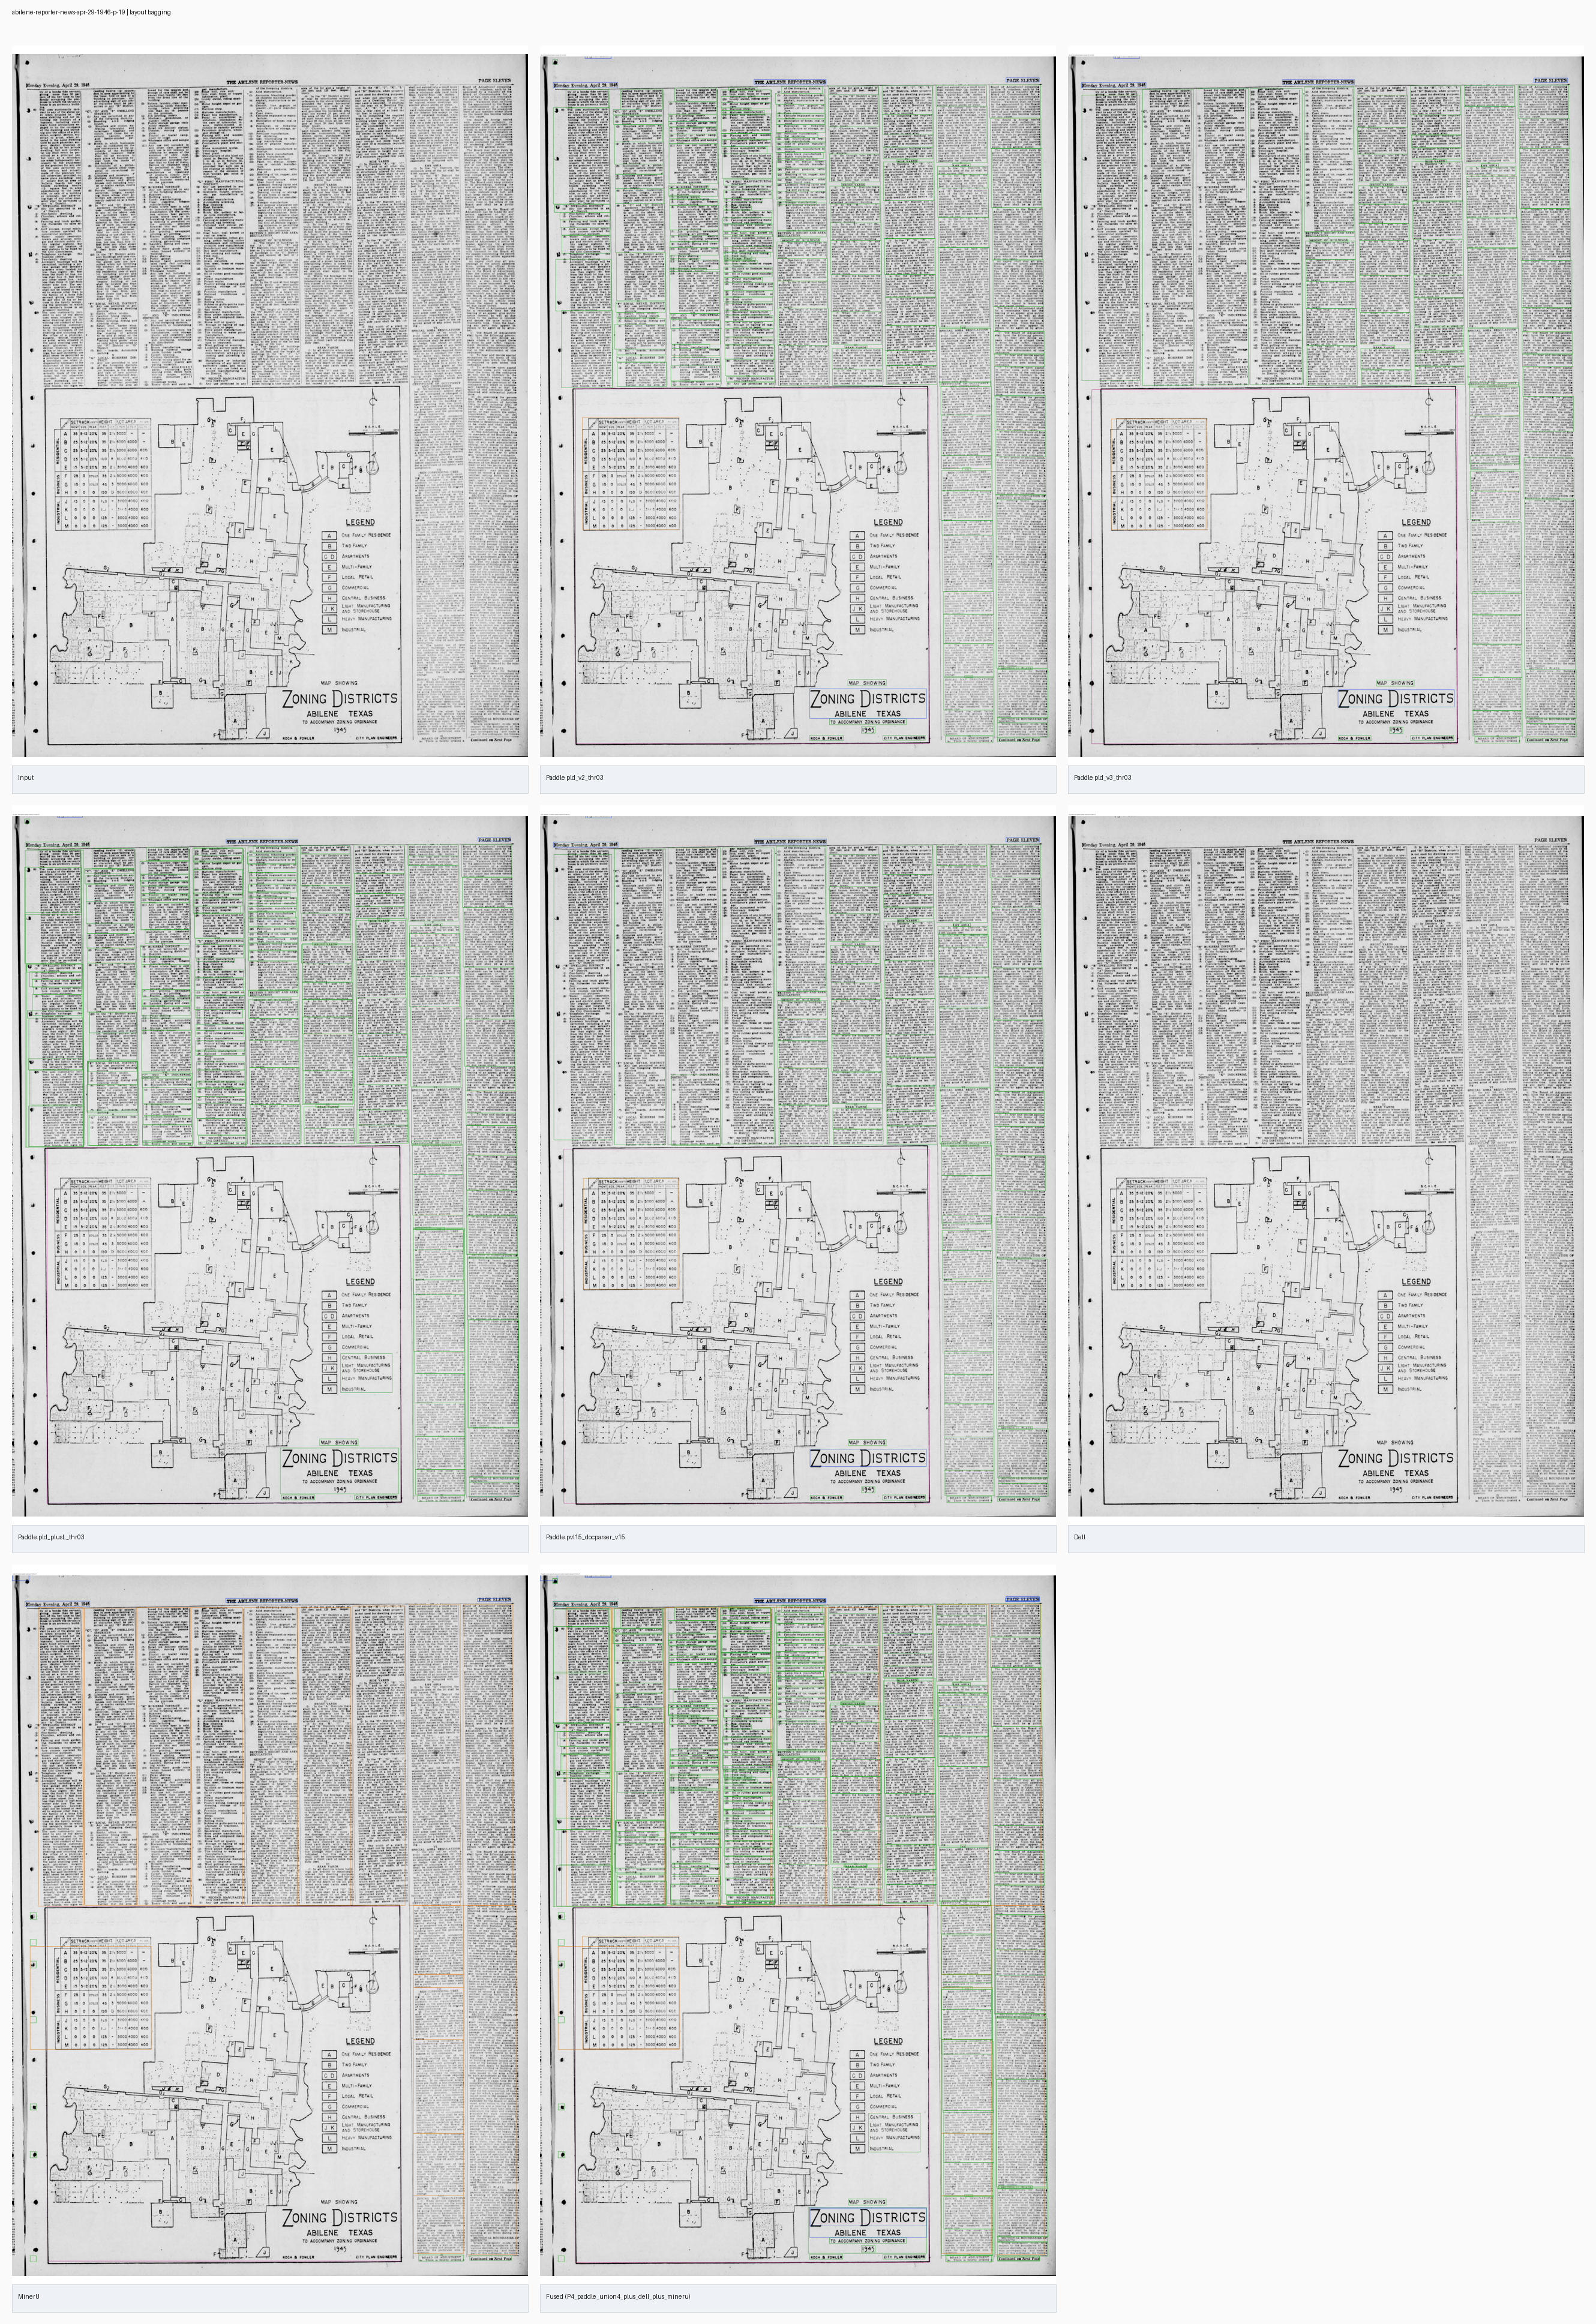
\includegraphics[width=0.92\textwidth]{images/mini_run/abilene_board.png}
\caption{Abilene full model board: Paddle4, Dell, MinerU, fused result.}
\end{figure}

\begin{figure}[h]
\centering
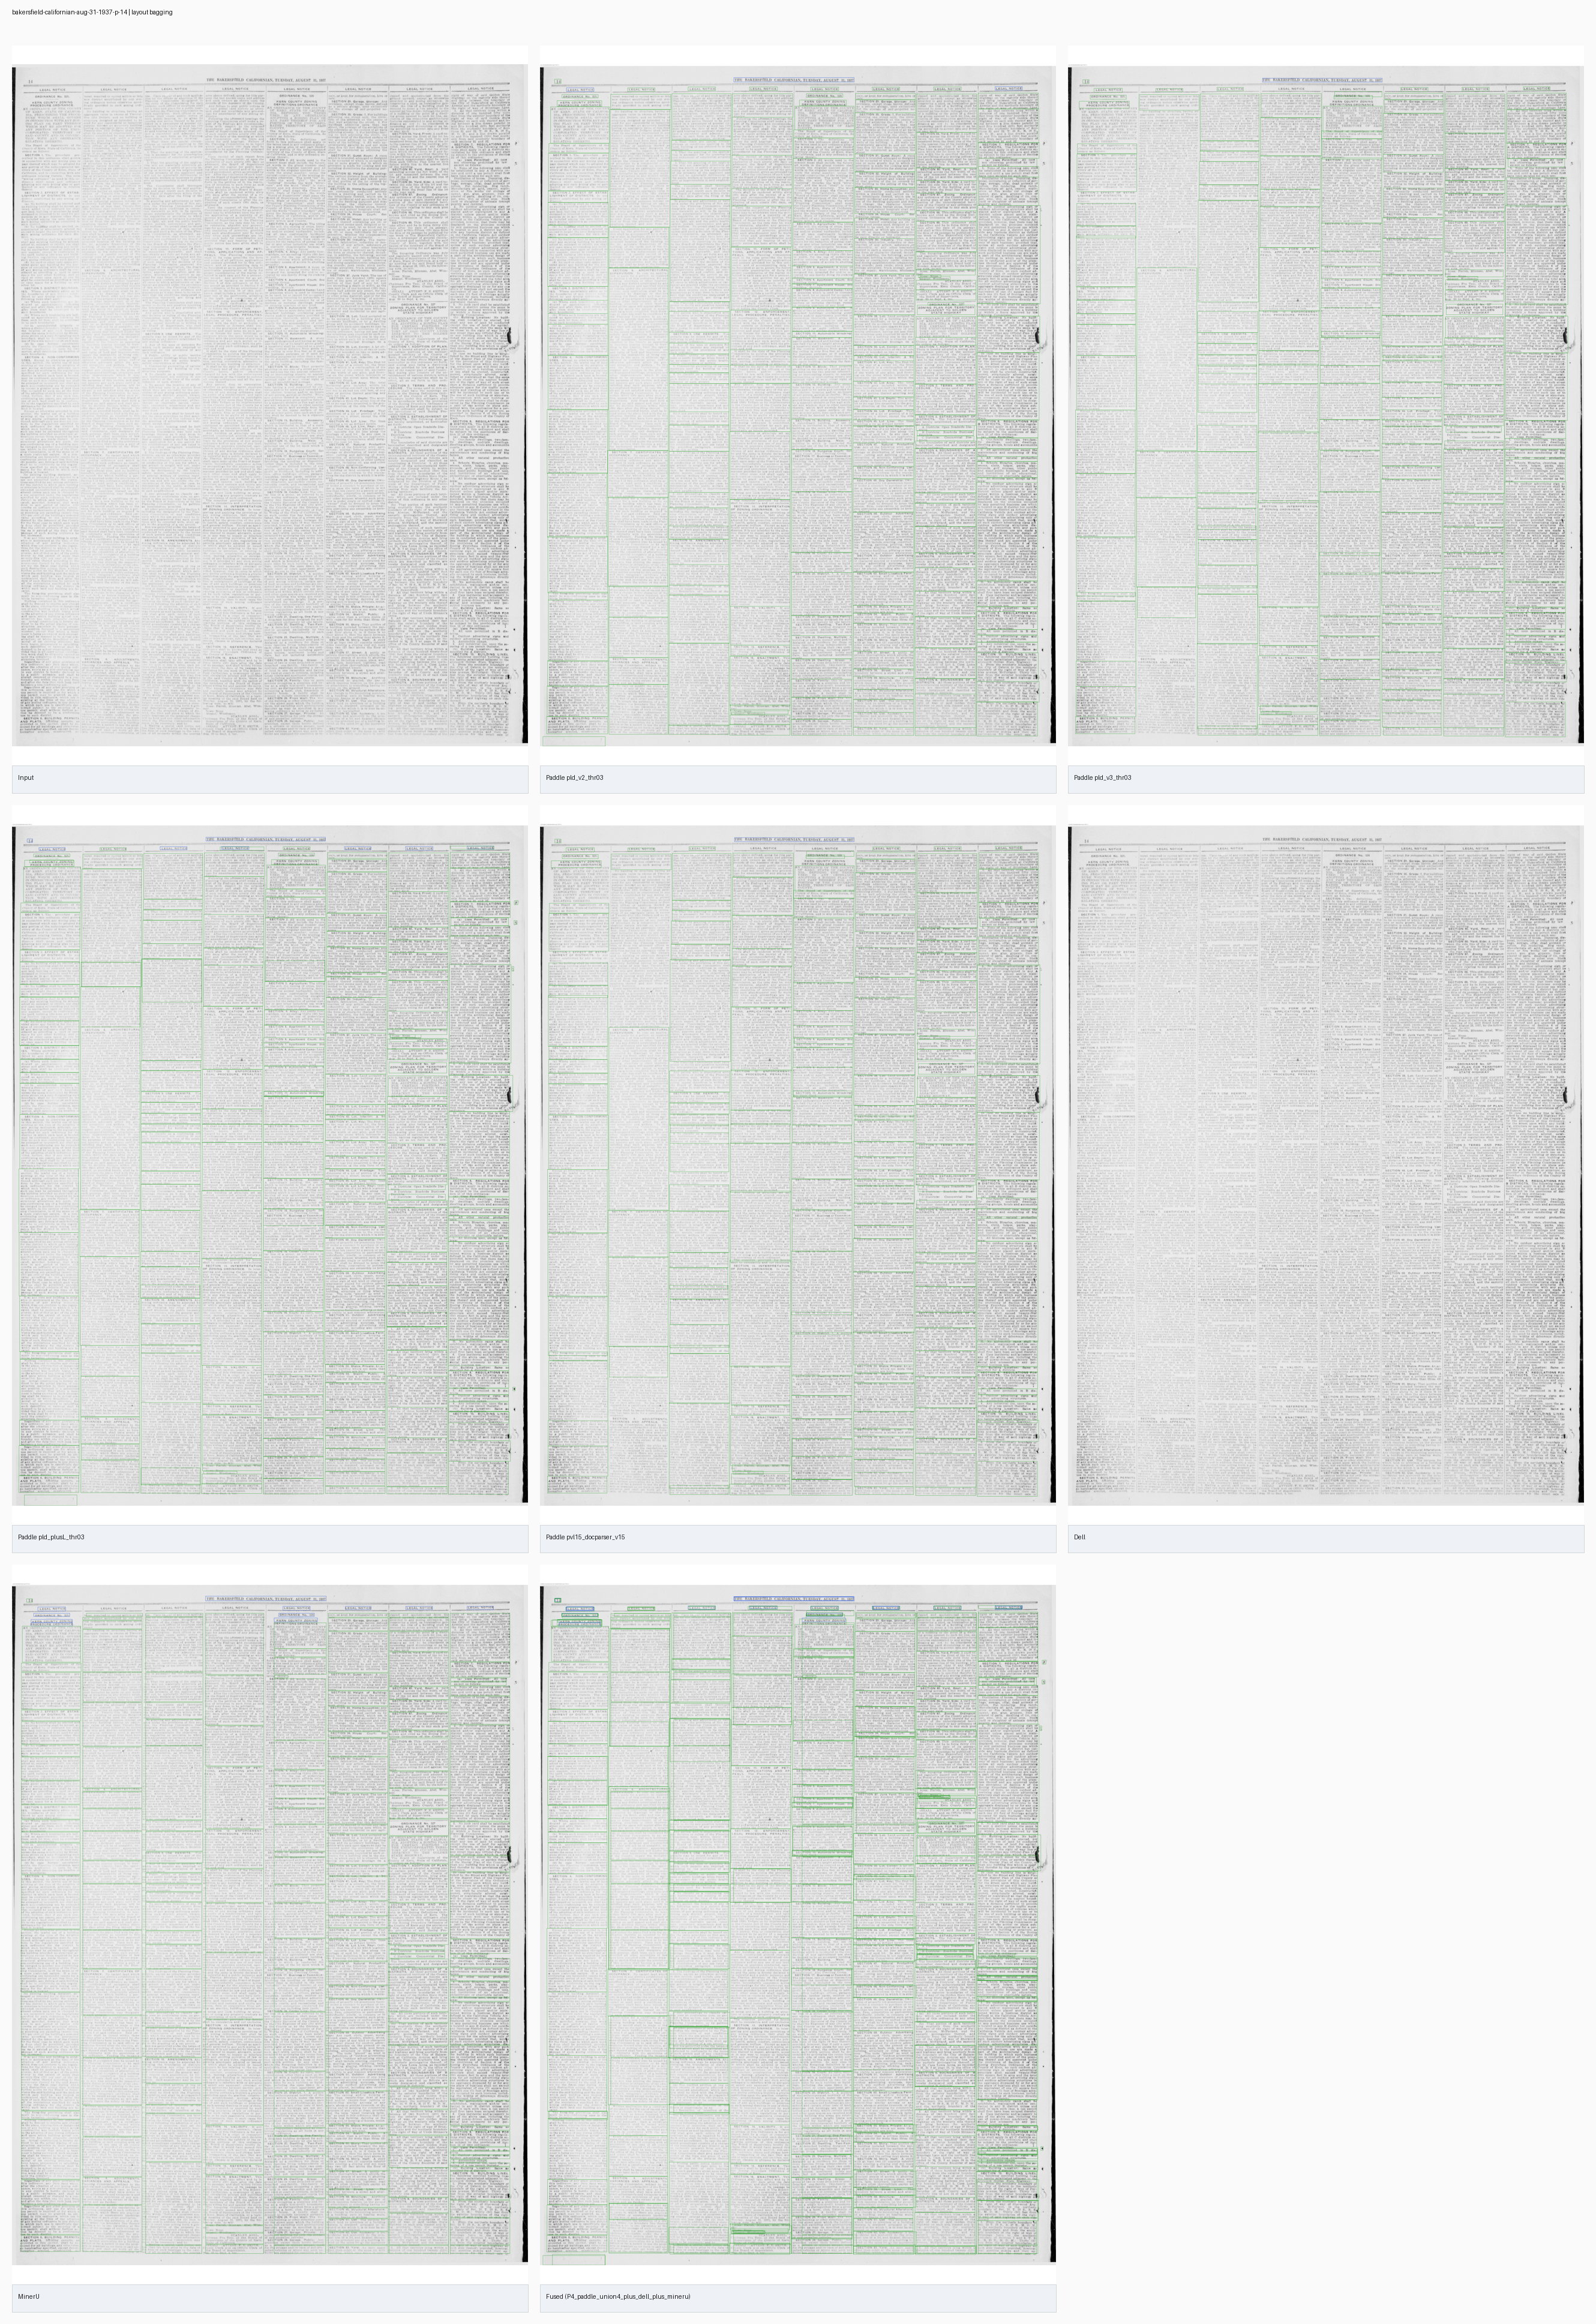
\includegraphics[width=0.92\textwidth]{images/mini_run/bakersfield_board.png}
\caption{Bakersfield full model board: Paddle4, Dell, MinerU, fused result.}
\end{figure}

\begin{figure}[h]
\centering
\includegraphics[width=0.92\textwidth]{images/mini_run/bakersfield_miner_delta.png}
\caption{Bakersfield with/without MinerU panel (\texttt{P2} vs \texttt{P4}).}
\end{figure}

\begin{figure}[h]
\centering
\includegraphics[width=0.92\textwidth]{images/mini_run/abilene_dell_layout.png}
\caption{Abilene Dell-only overlay after runner fix (non-empty output).}
\end{figure}

\clearpage
\subsection{Actual Metrics (from Run Artifacts)}
Variant leaderboard excerpt:
\begin{center}
\begin{tabular}{lrrr}
\toprule
Variant & Mean Base Recall & Mean Text Area & Mean Boxes \\
\midrule
\texttt{P2\_paddle\_union4\_plus\_dell} & 0.997774 & 0.737427 & 329.0 \\
\texttt{S1\_paddle\_best\_single} & 0.966463 & 0.698220 & 224.5 \\
\texttt{P4\_paddle\_union4\_plus\_dell\_plus\_mineru} & 0.997929 & 0.738797 & 404.5 \\
\bottomrule
\end{tabular}
\end{center}

Source leaderboard excerpt:
\begin{center}
\begin{tabular}{lrrr}
\toprule
Source & Mean Base Recall & Mean Text Area & Mean Boxes \\
\midrule
\texttt{pld\_plusL\_thr03} & 0.979841 & 0.698220 & 224.5 \\
\texttt{pld\_v2\_thr03} & 0.958174 & 0.689416 & 209.5 \\
\texttt{dell\_c0005\_i010} & 0.884912 & 0.584741 & 25.0 \\
\texttt{mineru25} & 0.473897 & 0.427513 & 125.0 \\
\bottomrule
\end{tabular}
\end{center}

\subsection{Dell Output Verification}
The corrected Dell runner produced non-empty outputs on both pages:
\begin{itemize}
  \item \texttt{abilene-reporter-news-apr-29-1946-p-19}: 23 boxes
  \item \texttt{bakersfield-californian-aug-31-1937-p-14}: 28 boxes
\end{itemize}
Counts were computed directly from the normalized Dell layout outputs for each page.

\subsection{Transcription Outputs}
Generated artifacts:
\begin{itemize}
  \item Transcription report (TSV)
  \item Combined transcript (TXT)
  \item Per-page:
    \begin{itemize}
      \item OCR metadata JSON
      \item OCR line JSON (page coordinates)
      \item Transcript-by-box JSON
      \item Transcript text
      \item OCR region overlay image
      \item OCR line overlay image
    \end{itemize}
\end{itemize}

\textbf{Transcription report excerpt:}
\begin{center}
\begin{tabular}{lrrrrr}
\toprule
Slug & Fused Boxes & OCR Regions & OCR Lines & Assigned Lines & Transcript Chars \\
\midrule
\texttt{abilene...p-19} & 331 & 54 & 3814 & 3814 & 32396 \\
\texttt{bakersfield...p-14} & 457 & 112 & 2871 & 2871 & 31760 \\
\bottomrule
\end{tabular}
\end{center}

\textbf{OCR region reduction in this run:}
\begin{itemize}
  \item \texttt{abilene...p-19}: 331 fused boxes $\rightarrow$ 54 OCR regions
  \item \texttt{bakersfield...p-14}: 457 fused boxes $\rightarrow$ 112 OCR regions
\end{itemize}

\subsection{OCR Output Examples}
The snippets below are direct transcript excerpts from the fused-layout OCR stage.

\textbf{Abilene excerpt:}
\begin{lstlisting}
Board of Adjustment consistin
of five (5) members.each to be
appointed by a majority of the
Board of Commissioners for a
term of two years and removabl
for cause by the appointing authority.
\end{lstlisting}

\textbf{Bakersfield excerpt (hard page, tiny legal text):}
\begin{lstlisting}
LEGAL NOTICE
The Planning Commission may adopt
such form as said Commission
deems advisable.
... (dense legal columns with OCR noise)
\end{lstlisting}

\begin{figure}[h]
\centering
\includegraphics[width=0.92\textwidth]{images/mini_run/abilene_ocr_regions_overlay.png}
\caption{Abilene OCR regions actually passed to Paddle OCR after overlap cleaning.}
\end{figure}

\begin{figure}[h]
\centering
\includegraphics[width=0.92\textwidth]{images/mini_run/abilene_ocr_lines_overlay.png}
\caption{Abilene remapped OCR line boxes on the original page.}
\end{figure}

\section{What to Inspect First}
\begin{enumerate}
  \item Full model board for each page
  \item With-vs-without MinerU comparison panel
  \item Variant leaderboard table
  \item Transcription report table
  \item Transcript text for each page
\end{enumerate}

\section{Reproducibility Notes}
\begin{itemize}
  \item The run records resolved configuration and resolved image manifest metadata.
  \item GPU inference and OCR were executed on compute-node-validated environments.
  \item Slurm wrappers re-install the editable package if runtime import roots drift from the project root.
  \item External-source fail-fast checks are now first-class:
  \texttt{dell.min\_nonempty\_pages} and \texttt{mineru.min\_nonempty\_pages}.
  If a source is empty across all processed pages, the run exits before fusion/review.
\end{itemize}

\appendix
\section{Full Verbatim OCR Transcripts}
This appendix includes the full per-page transcript outputs from the fused-layout OCR stage.

\subsection{Abilene (Full Transcript)}
\VerbatimInput[fontsize=\tiny]{appendix_transcripts/abilene_full_transcript.txt}

\subsection{Bakersfield (Full Transcript)}
\VerbatimInput[fontsize=\tiny]{appendix_transcripts/bakersfield_full_transcript.txt}

\end{document}
